\documentclass[10 pt,usenames,dvipsnames, oneside]{article}
\usepackage{../../../modelo-ensino-medio}


\begin{document}

\begin{center}
  \begin{minipage}[l]{3cm}
\includegraphics[width=2cm]{logo}    
\end{minipage}\hfill
\begin{minipage}[r]{.8\textwidth}
 {\Large \scshape Atividade: Gráficos, tabelas e fórmulas}  
\end{minipage}
\end{center}
\vspace{.2cm}

\ifdefined\prof
\begin{objetivos}
\item \textbf{LAF3} Calcular e interpretar a taxa de variação média de uma função em um intervalo dado, tanto algebricamente quanto a partir de dados gráficos ou de uma tabela, identificando tendências de crescimento e decrescimento.
\end{objetivos}

\begin{goals}
\begin{enumerate}

\item [OE1] Associar uma situação real a uma representação gráfica.

\item [OE2] Registrar com palavras o comportamento observado no gráfico.

\item [OE3] Construir tabelas a partir de informações dadas por uma situação.

\item [OE4] Confrontar o gráfico esboçado com a tabela construída.

\end{enumerate}

\tcblower

\begin{itemize}

\item Essa é uma atividade que inverte completamente a sequência tradicional fórmula $\rightarrow$
tabela $\rightarrow$ gráfico.
\item Esperamos que essa atividade forneça uma sensação “qualitativa” da natureza das
funções.

\item Para a primeira situação descrita é possível que alguns estudantes apresentem um
gráfico como o seguinte:

\begin{figure}[H]
\centering
\begin{tikzpicture}[xscale=.75, scale=.7]

\draw [->] (0,0) -- (16,0) node [below left, yshift=-.25cm] {Tempo (meses)};
\draw [->] (0,0) -- (0,9) node [above left, xshift=-.75cm, rotate=90] {Custo (reais)};
\draw [help lines] (0,0) grid (16,9);

\foreach \x in {80,160,...,800} \node [left] at (0,\x*0.01) {\x};
\foreach \x in {5,10,15} \node [below] at (\x,0) {\x};

\clip (0,0) rectangle (15,9);
\draw[domain=1:13, thick, session3] plot (\x,{0.8*\x-0.8});
\end{tikzpicture}
\end{figure}

Caso apareça uma solução como esta, sugerimos encaminhar as discussões destacando
os seguintes fatos: o domínio a ser considerado é um conjunto discreto; o gráfico acima
representa uma situação em que considera-se o custo sendo acumulado mês a mês.

\item Encontrar uma fórmula será o principal obstáculo. Neste ponto pode ajudar bastante se
primeiro for solicitado aos estudantes que falem e depois registrem por escrito o
método que eles usaram para construir as tabelas de valores. A observação de
tendências e padrões a partir das tabelas deverá facilitar a obtenção das expressões
algébricas.

\item Os estudantes podem ter um pouco mais de dificuldade para responder ao item (d). Isso
não é grave nesse momento, e de certa forma, contribui para o entendimento que nem
sempre precisamos (ou conseguiremos) encontrar uma expressão matemática que
relacione as grandezas, mas mesmo assim podemos ter ideias qualitativas sobre o
comportamento e as variações.

\end{itemize}
\end{goals}

\bigskip
\begin{center}
{\large \scshape Atividade}
\end{center}
\fi

Para cada uma das situações a seguir:
\begin{enumerate}
\item Responda à pergunta fazendo o esboço de um gráfico
\item Descreva com palavras a forma do seu gráfico
\item Verifique seu gráfico construindo uma tabela de valores. Caso seja necessário, refaça seu esboço
\item Tente encontrar uma expressão algébrica que descreva a situação
\end{enumerate}

\begin{description}\item[TV por assinatura]
Uma empresa de TV por assinatura cobra R\$ 80,00 por mês por um determinado pacote de canais. Uma oferta para novos assinantes oferece o primeiro mês gratuitamente. Como irá variar o custo da assinatura conforme o período de tempo aumenta?
\item[Valor de mercado de um carro]
Comprei um carro por R\$ 65.000,00 e seu valor está depreciando a uma taxa de 20\% ao ano. Isso significa que depois de um ano seu valor era de $60.000\times 0,8=52.000$, depois de dois anos, $52.000\times 0,8=41.600$ e assim por diante. Como o valor de mercado desse carro continuará a mudar?
\item[Subindo uma escada]
Uma passada normal tem em média 60cm de compreimento. Ela deve diminuir 2cm para cada 1cm que o pé é levantado quando estamos subindo os degraus de uma escada. Seguindo esse princípio, como deve varia o comprimento da passada com a altura de um degrau?
\item[Polígonos Regulares]
Como a medida de um dos ângulos internos depende do número de lados de um polígono regular?
\end{description}

\begin{table}[H]
\centering
\setlength\tabcolsep{5pt}
\begin{tabu} to \textwidth{*{8}{c}}
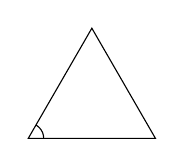
\begin{tikzpicture}[scale=.7*1.333]

% \draw circle (1.333*0.5cm);
\foreach \x/\y in {a/90:1,b/210:1,c/330:1}
 \coordinate (\x) at (\y);

\clip[draw] (a) -- (b) -- (c) -- cycle;
\draw (b) circle (6pt);
\end{tikzpicture} &

\begin{tikzpicture}[scale=.7*sqrt(2)]
% \draw circle (1.414213562*0.5cm);
\foreach \x/\y in {a/45:1,b/135:1,c/225:1,d/315:1} \coordinate (\x) at (\y);


\clip[draw] (a) -- (b) -- (c) -- (d) -- cycle;
\draw (225:1) circle (6pt);

\end{tikzpicture} &

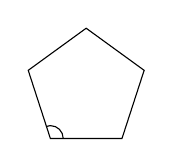
\begin{tikzpicture}[scale=.7*1.1056]
% \draw circle (1cm);
\foreach \x/\y in {a/90:1,b/90+72:1,c/90+72*2:1,d/90+72*3:1,e/90+72*4:1} \coordinate (\x) at (\y);


\clip[draw] (a) -- (b) -- (c) -- (d) -- (e) -- cycle;
\draw (90+72*2:1) circle (6pt);


\end{tikzpicture} &

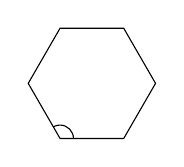
\begin{tikzpicture}[scale=.7*1.155]
% \draw circle (1cm);
\foreach \x/\y in {a/0:1,b/60:1,c/60*2:1,d/60*3:1,e/60*4:1,f/60*5:1} \coordinate (\x) at (\y);


\clip[draw] (a) -- (b) -- (c) -- (d) -- (e) -- (f) -- cycle;
\draw (60*4:1) circle (6pt);


\end{tikzpicture} &

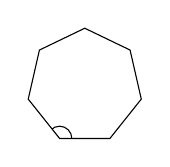
\begin{tikzpicture}[scale=.7*1.052]
% \draw circle (1cm);
\foreach \x/\y in {a/90:1,b/90+51.428571429:1,c/90+51.428571429*2:1,d/90+51.428571429*3:1,e/90+51.428571429*4:1,f/90+51.428571429*5:1, g/90+51.428571429*6:1} \coordinate (\x) at (\y);


\clip[draw] (a) -- (b) -- (c) -- (d) -- (e) -- (f) -- (g) -- cycle;
\draw (90+51.428571429*3:1) circle (6pt);


\end{tikzpicture} &

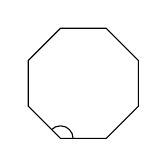
\begin{tikzpicture}[scale=.7*1.082]
% \draw circle (1cm);
\foreach \x/\y in {a/22.5:1,b/22.5+45*1:1,c/22.5+45*2:1,d/22.5+45*3:1,e/22.5+45*4:1,f/22.5+45*5:1, g/22.5+45*6:1,h/22.5+45*7:1} \coordinate (\x) at (\y);


\clip[draw] (a) -- (b) -- (c) -- (d) -- (e) -- (f) -- (g) -- (h) -- cycle;
\draw (22.5+45*5:1) circle (6pt);


\end{tikzpicture} &

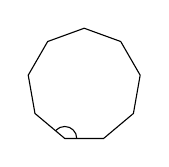
\begin{tikzpicture}[scale=.7*1.031]
% \draw circle (1cm);
\foreach \x/\y in {a/90:1,b/90+40*1:1,c/90+40*2:1,d/90+40*3:1,e/90+40*4:1,f/90+40*5:1, g/90+40*6:1,h/90+40*7:1,i/90+40*8:1} \coordinate (\x) at (\y);


\clip[draw] (a) -- (b) -- (c) -- (d) -- (e) -- (f) -- (g) -- (h) -- (i) -- cycle;
\draw (e) circle (6pt);



\end{tikzpicture} &

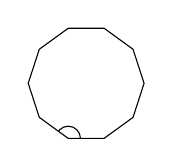
\begin{tikzpicture}[scale=.7*1.051]
% \draw circle (1cm);
\foreach \x/\y in {a/0:1,b/36*1:1,c/36*2:1,d/36*3:1,e/36*4:1,f/36*5:1, g/36*6:1,h/36*7:1,i/36*8:1,j/36*9:1} \coordinate (\x) at (\y);


\clip[draw] (a) -- (b) -- (c) -- (d) -- (e) -- (f) -- (g) -- (h) -- (i) -- (j) -- cycle;
\draw (h) circle (6pt);


\end{tikzpicture} 

\end{tabu}
\end{table}


\textbf{Sugestão:} Você pode calcular a soma de todos os ângulos internos de cada um dos polígonos subdividindo-os em triângulos, por exemplo: 

\medskip
\begin{minipage}{0.45\textwidth}
\centering
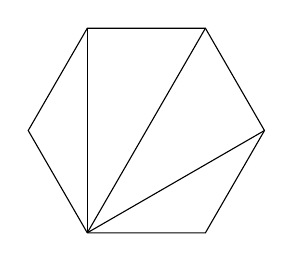
\begin{tikzpicture}[scale=1.5]
\foreach \x/\y in {a/0:1,b/60:1,c/60*2:1,d/60*3:1,e/60*4:1,f/60*5:1} \coordinate (\x) at (\y);


\clip[draw] (a) -- (b) -- (c) -- (d) -- (e) -- (f) -- cycle;

\draw (e) -- (a);
\draw (e) -- (b);
\draw (e) -- (c);

\end{tikzpicture}
\end{minipage}
\begin{minipage}{0.45\textwidth}
Soma dos ângulos internos: $4\times180^{\circ}=720^{\circ}$
\end{minipage}

\ifdefined\prof

\begin{solucao}

\begin{enumerate}

\item \textbf{TV por assinatura}

\begin{center}
\begin{tikzpicture}[every node/.style={black}, every path/.style={black},scale=.7]
\draw [->] (-.5,0) -- (12,0) node [below left, yshift=-.5cm] {Tempo (meses)};
\draw [->] (0,-.5) -- (0,9) node [above left,rotate=90, yshift=.5cm] {Custo da mensalidade (R\$)};
\draw [help lines] (0,0) grid (12,9);
\foreach \x in {1,...,11} \node [below] at (\x,0) {\x};
\node [left] at (0,8) {80};
\node [left] at (0,4) {40};
\node [below left] at (0,0) {0};

\fill [session3] (1,0) circle (3pt);
\foreach \x in {2,...,10} \fill [session3] (\x,8) circle (3pt);
\end{tikzpicture}
\end{center}

\textbf{Valor de mercado de um carro}

\begin{center}
\begin{tikzpicture}[every node/.style={black}, every path/.style={black},scale=.7]
\draw [->] (-.5,0) -- (16,0) node [below left, yshift=-.5cm] {Tempo (anos)};
\draw [->] (0,-.5) -- (0,8) node [above left,rotate=90, yshift=1.1cm] {Valor do carro (R\$)};
\draw [help lines] (0,0) grid (16,8);
\foreach \x in {1,...,16} \node [below] at (\x,0) {\x};
\node [left] at (0,5) {50.000};
\node [left] at (0,2.5) {25.000};
\node [left] at (0,7.5) {75.000};
\node [below left] at (0,0) {0};

\foreach \x/\y in {0/6.5,1/6.5*.8,2/6.5*.8^2,3/6.5*.8^3,4/6.5*.8^4,5/6.5*.8^5,6/6.5*.8^6,7/6.5*.8^7,8/6.5*.8^8,9/6.5*.8^9,10/6.5*.8^10,11/6.5*.8^11,12/6.5*.8^12,13/6.5*.8^13,14/6.5*.8^14,15/6.5*.8^15} \fill [session3] (\x,\y) circle (3pt);

\draw [domain=0:15, session3, dashed] plot (\x,{6.5*0.8^\x});
\end{tikzpicture}
\end{center}

\textbf{Subindo uma escada}

\begin{center}
\begin{tikzpicture}[every node/.style={black}, every path/.style={black},scale=.7]
\draw [->] (-.5,0) -- (15,0) node [below left, yshift=-.5cm] {Altura do degrau (cm)};
\draw [->] (0,-.5) -- (0,6) node [above left,rotate=90, yshift=.5cm] {Passada (cm)};
\draw [help lines] (0,0) grid (15,6);
\foreach \x/\y in {2/5,4/10,6/15,8/30,10/20,12/25,14/30} \node [below] at (\x,0) {\y};
\foreach \x/\y in {1/20,2/40,3/60,4/80,5/100} \node [left] at (0,\x) {\y};

\draw [thick, session3] (0,3) -- (14,0);
\fill [session3] (0,3) circle (3pt);

\node [below left] at (0,0) {0};


\end{tikzpicture}
\end{center}

\textbf{Polígonos regulares}

\begin{center}
\begin{tikzpicture}[every node/.style={black}, every path/.style={black},scale=.7,yscale=.5]
\draw [->] (-.5,0) -- (14,0) node [below left, yshift=-.5cm] {Número de lados};
\draw [->] (0,-.5) -- (0,17) node [above left,rotate=90, yshift=.5cm] {Tamanho de cada ângulo (graus)};
\draw [help lines] (0,0) grid (14,16);
\foreach \x in {2,4,...,14} \node [below] at (\x,0) {\x};
\foreach \x in {4,8,12,16} \node [left] at (0,\x) {\x0};

\foreach \x/\y in {3/6,4/9,5/10.8,6/12,7/12.86,8/13.5,9/14,10/14.4,11/14.727} \node [fill,circle, inner sep=1.5pt, session3] at (\x,\y) {};

\node [below left] at (0,0) {0};
\draw [dashed, session3, domain=3:11] plot (\x,{18-36/\x});


\end{tikzpicture}
\end{center}

\item \textbf{TV por assinatura} - No primeiro mês o custo é zero, nos meses seguintes é cobrado o valor fixo de R\$ 80,00, por isso o gráfico é um conjunto de pontos distribuídos sobre uma reta que intercepta o eixo $y$ no ponto $(0,80)$.

\textbf{Valor de mercado de um carro} - A cada ano o valor de mercado do automóvel vai diminuindo, no entando, a desvalorização sofrida no ano anterior será sempre maior do que a desvalorização observada no ano seguinte. Dessa forma, o gráfico terá a forma de uma curva suave que se inicia no ponto $(0,65.000) $ e se aproxima de zero na medida em que o tempo em anos aumenta.

\textbf{Subindo uma escada} - Temos uma diminuição uniforme de $2$ cm no comprimento da passada cada vez que aumentamos $1$ cm a altura do degrau. Dessa forma o gráfico será uma reta com ponto inicial em $(0,60)$ e ponto final $(30,0)$, uma vez que para um degrau de $30$ cm de altura será de $0$ cm.

\textbf{Polígonos regulares} - A medida do ângulo interno de um pólígono regular aumenta à medida em que aumentamos o número de lados. Esse aumento, no entanto, não é uniforme, uma vez que para cada lado a mais considerado o aumento corresponde percebido no ângulo interno é cada vez menor. Dessa forma o ângulo interno cresce lentamente conforme o número de lados do polígono regular aumenta.

\item \textbf{TV por assinatura}



\begin{tabu} to \textwidth{|c|c|}
\hline
\thead
Tempo (meses) & Custo da assinatura (R\$) \\
\hline
1 & 0 \\
\hline
2 & 80 \\
\hline
3 & 80 \\
\hline
2 & 80 \\
\hline
$\vdots$ & $\vdots$ \\
\hline
\end{tabu}
\newpage


\textbf{Valor de mercado de um carro}


\begin{tabu} to \textwidth{|c|c|}
\hline
\thead
Tempo (anos) & Valor de mercado do carro (R\$) \\
0 & 65.000,00 \\
\hline
1 & 52.000,00 \\
\hline
2 & 41.600,00 \\
\hline
3 & 33.280,00 \\
\hline
$\vdots$ & $\vdots$ \\
\hline
\end{tabu}
\vspace{1em}

\textbf{Subindo uma escada}


\begin{tabu} to \textwidth{|c|c|}
\hline
\thead
Altura do degrau (cm) & Comprimento da passada (cm) \\
0 & 60 \\
\hline
1 & 58 \\
\hline
2 & 56 \\
\hline
3 & 54 \\
\hline
$\vdots$ & $\vdots$ \\
\hline
\end{tabu}

\vspace{1em}
\textbf{Polígonos regulares}


\begin{tabu} to \textwidth{|c|c|}
\hline
\thead
Número de lados & Tamanho de cada ângulo (graus) \\
3 & 60 \\
\hline
4 & 90 \\
\hline
5 & 108 \\
\hline
6 & 120 \\
\hline
7 & 128,6 \\
\hline
8 & 135 \\
\hline
$\vdots$ & $\vdots$ \\
\hline
\end{tabu}


\item \textbf{TV por assinatura}

\[C(t)
\begin{cases}
0,\text{ se } t=1\\
80,\text{ se } t=2,3,4,...
\end{cases}
\]

\begin{center}
$C$ - valor fixo da mensalidade em reais, $t$=período de assinatura em meses.
\end{center}

\textbf{Valor de mercado de um carro}
\begin{equation*}
V(t)=65.000\times 0,8^t
\end{equation*}
\begin{center}
$V$ = valor do carro em reais, $t$= idade do carro em anos.
\end{center}

\textbf{Subindo uma escada}
\begin{equation*}
P(h)=60-2h
\end{equation*}
\begin{center}
$P$ = medida passada em centímetros, $h$=altura do degrau em centímetros.
\end{center}

\textbf{Polígonos regulares}
\begin{equation*}
A(n)=180-\frac{360}{n}
\end{equation*}
\begin{center}
$A$=medida de cada ângulo interno, $n$=número de lados do polígono regular.
\end{center}
\end{enumerate}
\end{solucao}
\fi

\end{document}